\documentclass[a4paper]{article}

\usepackage{geometry}
\geometry{margin=2cm}

\usepackage{graphicx}
\usepackage{subfig}
\usepackage{dsfont}
\usepackage{amsmath}
\usepackage{url}

\newcommand{\tr}[1]{\text{trace}(#1)}
\newcommand\norm[2]{\left\lVert#1\right\rVert _{#2}}

\begin{document}

	\title{A convex optimization approach to PCA}
	\author{Vincenzo Bazzucchi}
	\maketitle

\begin{abstract}
Principal Component Analysis is a fundamental technique in statistics and unsupervised dimensionality reduction. In this paper \textbf{Principal Component Pursuit (PCP)} is explored, a convex problem whose solution separates a lower rank representation and the sparse noise from a given data matrix $M$
\end{abstract}

\section{Introduction}
Classical Principal Component analysis of the matrix $M\in \mathds{R}^{n \times m}$ can be formulated as the following problem:
\begin{equation}
\begin{aligned}
& \underset{L}{\text{minimize}}
& & ||M-L|| \\
& \text{subject to}
& & \text{rank}(L) \leq \lambda
\end{aligned}
\end{equation}

However this approach is sensitive to corrupted measurements which are very common in imge processing, web data analysis ad bioinformatics just to quote a few.
\cite{RPCA} introduced \textbf{Principal Component Pursuit}:
\begin{equation}
\label{pcp}
\begin{aligned}
& \underset{L, S}{\text{minimize}}
& & \norm{L}{*} + \lambda\norm{S}{1} \\
& \text{subject to}
& & L + S = M
\end{aligned}
\end{equation}
Where $L$ is a lower rank matrix, $S$ a sparse matrix, $\norm{M}{*} = \sum_i \sigma_i(M)$ is the nuclear norm (the sum of the eigenvalues) of the matrix $M$ and $\norm{M}{1} = \sum_{i,j} |M_{ij}|$

The first obvious remark is that the the problem \ref{pcp} is convex: all the $p$-norms are convex functions and the constraint is linear.

\section{A Semi-Definite Programming Problem}
\ref{pcp} can be rewritten by leveraging that $M = L + S \Leftrightarrow L = M - S$.
\begin{equation}
\label{pcp1var}
\begin{aligned}
& \underset{L}{\text{minimize}}
& & ||M - S||_* + \lambda||S||_1 \\
\end{aligned}
\end{equation}

The optimal value of \ref{pcp} then becomes
\begin{equation}
\begin{aligned}
p^* & = \min_S \norm{M - S}{*} + \lambda \norm{S}{1} \\
    & = \min_S \max_{Y, Z} \tr{Y^T(M - S)} + \tr{Z^T S} : \norm{Y}{2}\leq 1, \norm{Z}{\infty} \leq \lambda \\
    & = \max_{Y, Z} \min_S \tr{Y^T(M - S)} + \tr{Z^T S} : \norm{Y}{2}\leq 1, \norm{Z}{\infty} \leq \lambda \\ 
    & = \max_Y \tr{Y^TM} : \norm{Y}{2}\leq 1, \norm{Y}{\infty} \leq \lambda \\ 
\end{aligned}
\end{equation}
Where $Y\in \mathds{R}^{n\times n}$ is the \textit{Lagrange multiplier}

The condition $||Y||\leq 1$ is equivalent to $I  - YY^T \succeq 0$ which can be written as a linear matrix inequality using Shcur complements:
$$ X = \begin{bmatrix} I & Y \\ Y^T & I \end{bmatrix} \succeq 0$$
This problem can therefore be expressed as an SDP:
\begin{equation}
\label{sdp}
\begin{aligned}
& \underset{Y}{\text{maximize}}
& & \tr{Y^T M}\\
& \text{subject to}
& & \begin{bmatrix} I & Y \\ Y^T & I \end{bmatrix} \succeq 0 \\
& & & \lambda \leq Y_{ij} \leq \lambda, 1 \leq i \leq j \leq n
\end{aligned}
\end{equation}

\section{The Alternating Direction Method}
First let's define the augmented Lagrangian:
$$l(L,S, Y) = ||L||_* + \lambda ||S||_1 + \tr{Y^T (M - L - S)} + \frac{\mu}{2} ||M - L - S||^2_F$$
Then iteratively solve the problem is solved by optimizing the primal variables and then by using the new values of the primal variables to update the dual variable:
\begin{enumerate}
    \item $L_k, S_k = \arg \min_{L, S} l(L, S, Y_k)$
    \item $Y_k = Y_k + \mu ( M - L_k - S_k)$
\end{enumerate}
To compute $L_k, S_k$ \cite{RPCA} introduced
\begin{itemize}
    \item the \textbf{shrinkage} operator: $\mathcal{S}_\tau(x) = \text{sgn}(x)\max(|x|-\tau, 0)$
    \item the \textbf{thresholding} operator: $\mathcal{D}_\tau (A) = U \mathcal{S}_\tau(\Sigma) V^T$ where $A = U \Sigma V^T$ is a SVD decomposition of $A$
\end{itemize}
Then
$$\arg \min _L l(S_k, L, Y_k) = \mathcal{S}_{\lambda \mu^{-1}} (M - L + \mu^{-1}Y_k)$$
$$\arg \min _S l(S, L_k, Y_k) = \mathcal{D}_{\mu^{-1}} (M - S + \mu^{-1}Y_k)$$

Using $\mu = \frac{nm}{4\norm{M}{1}}$, $\lambda = \frac{1}{\sqrt{\max(n, m)}}$ and stopping when $\norm{M-L-S}{F} \leq 10^{-7} \norm{M}{F}$

An implementation of this algorithm in Python can be found in the \texttt{robust\_pca.py} file.

\section{Recovering corrupted images}
RPCA is often used to recover data from corrupted matrices. \cite{RPCA} shows this generating random matrices and then perturbing them before applying the algorithm. In some papers using Robust PCA that were analyzed, the algorithm is used to extract the background from video surveillance footage (\cite{RPCA}, \cite{fast}) or for data analysis \cite{data}.

For this project, I attempted to apply this powerful algorithm to a type of data mentioned in the original paper: images.
Some random uniform noise was generated and applied to random pixels of the red, green and blue channels of an image. Then robust PCA was executed on the perturbed images and the lower rank matrix was compared to the original image.
The experiment was replicated varying the ratio of perturbed pixels. The results are displayed in figure \ref{experiment} while the code necessary to corrupt and recover the images is in \texttt{image\_recovery.py}.

The accuracy of the recovery was measured by by computing the Pearson correlation coefficient\footnote{\url{https://en.wikipedia.org/wiki/Pearson_correlation_coefficient#For_a_sample}} between the original image and the corrupted image channel by channel and by averaging over the three channels. The same computation is performed on the recovered image. The similarities values are also shown in Figure \ref{experiment}. As a reminder, the Pearson correlation coefficient value are in the range $[-1, 1]$ where a value close to $1$ indicates high similarity. The experiment can be run executing \texttt{run.py}

\begin{figure}
    \centering
    \begin{tabular}{cc}
        \multicolumn{2}{c}{Original image} \\
        \multicolumn{2}{c}{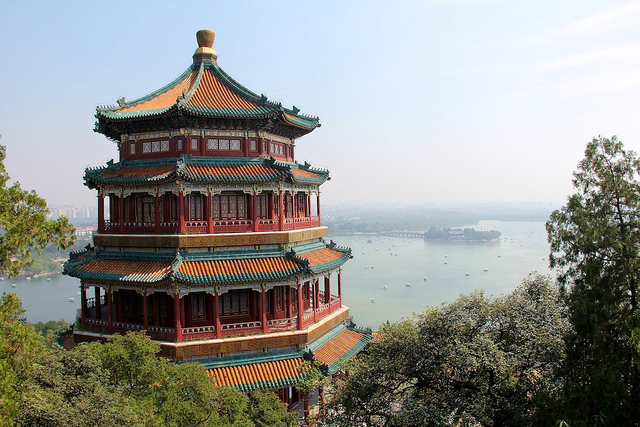
\includegraphics[width=45mm]{original.png} }\\
        \multicolumn{2}{c}{30\% altered pixels} \\
        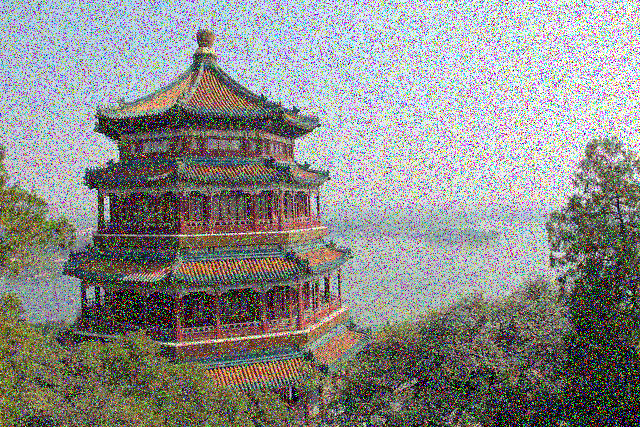
\includegraphics[width=45mm]{perturbed-3} & 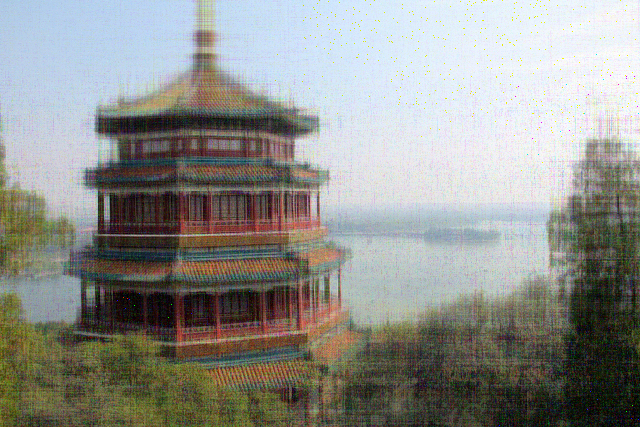
\includegraphics[width=45mm]{restored-3} \\
        $0.72$ & $0.96$ \\
        \multicolumn{2}{c}{20\% altered pixels} \\
        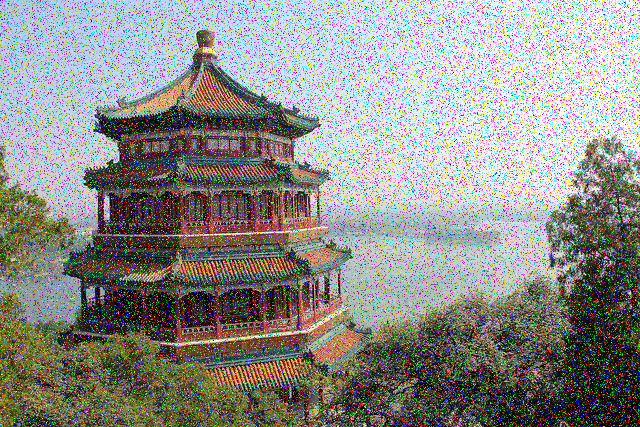
\includegraphics[width=45mm]{perturbed-2} & 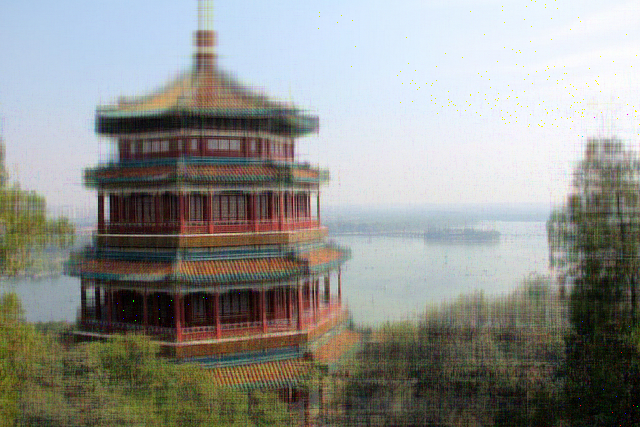
\includegraphics[width=45mm]{restored-2} \\
        $0.82$ & $0.96$ \\
        \multicolumn{2}{c}{10\% altered pixels} \\
        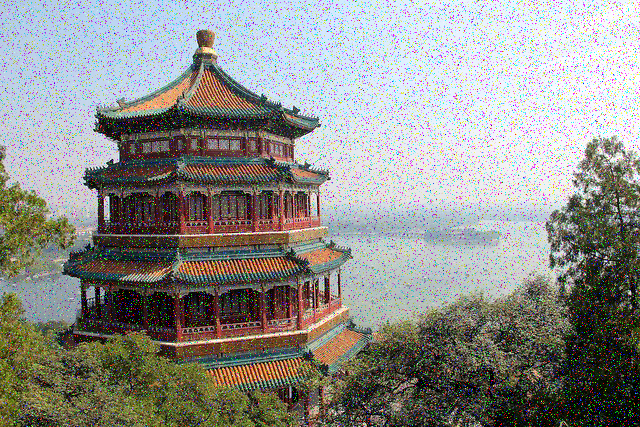
\includegraphics[width=45mm]{perturbed-1} & 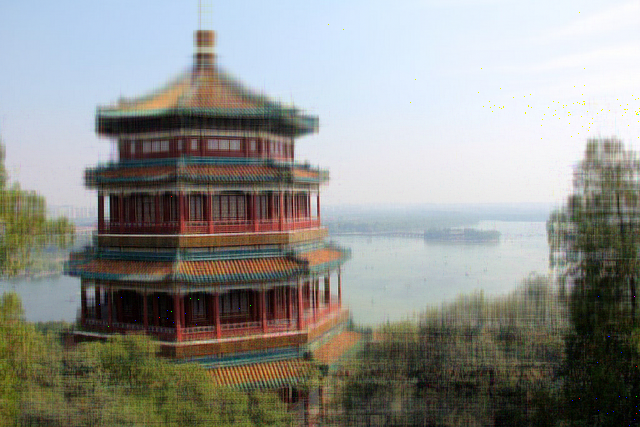
\includegraphics[width=45mm]{restored-1} \\
        $0.91$ & $0.97$ \\
        \multicolumn{2}{c}{5\% altered pixels} \\
        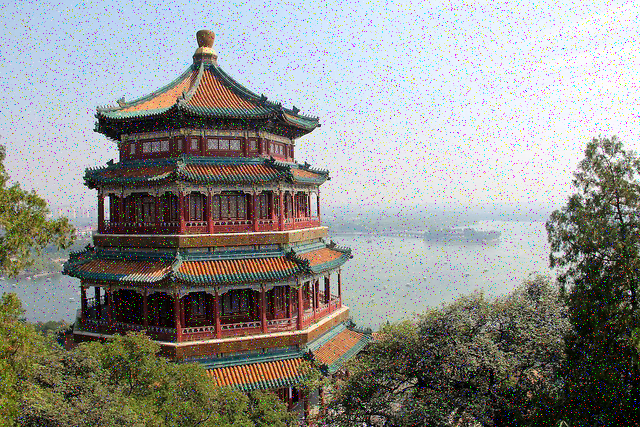
\includegraphics[width=45mm]{perturbed-05} & 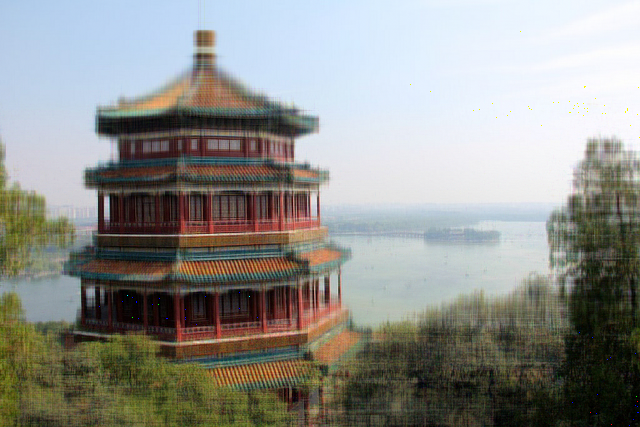
\includegraphics[width=45mm]{restored-05} \\
        $0.96$ & $0.97$ \\
    \end{tabular}
    \caption{Recovering a corrupted image. On the left the corrupted images with different ratios of altered pixels, on the recovered image}
    \label{experiment}
\end{figure}

\begin{thebibliography}{5}
    \bibitem{RPCA}
    Candés, E. J., Li, X., Ma, Y. and Wright, J. (2009). \em{Robust principal component analysis?}

    \bibitem{fast}
    Pupusha, I. (2011). \em{Fast automatic background extraction via Robust PCA}

    \bibitem{data}
    Fan, J., Sun, Q., Zhou, W.X., Zhu, Z. \em{Principal component analysis for big data}
\end{thebibliography}
\end{document}

